%%%%%%%%%%%%%%%%%%%%%%%%%%%%%%%%%%%%%%%%%%%%%%%%%%%%%%%%%%%%%%%%%%%%%%%%%%%%%%%%%%%%%%%%%%%%%%%%%%%%%%%%%%%%%%%%%%%%%%%%%%%%%%%%%%%%%%%%%%%%
% Dies ist ein Kommentar, er wird bei der pdf-Erzeugung ignoriert.

% Dies ist die einfachste Form einer LaTex-Vorlage für den Gebrauch im physikalischen Praktikum I mit einigen Kommentaren. Mit der Zeit können Sie diese Vorlage gerne verfeinern oder sich eine andere wählen. Die Kapitel beinhalten teilweise Beispiele wie die Darstellung von Grafiken/Tabellen oder mathematischen Formeln sowie Referenzen/Zitationen. 

%%%%%%%%%%%%%%%%%%%%%%%%%%%%%%%%%%%%%%%%%%%%%%%%%%%%%%%%%%%%%%%%%%%%%%%%%%%%%%%%%%%%%%%%%%%%%%%%%%%%%%%%%%%%%%%%%%%%%%%%%%%%%%%%%%%%%%%%%%%%

\documentclass[a4paper,12pt,bibtotocnumbered]{scrartcl} %Die Dokumentenklasse. In "Word" wäre das die Dukumentenvorlage

%Einbidung der Pakete. Diese Liste kann sehr lang werden...
\usepackage[utf8]{inputenc} %Zeichencodierung des LaTeX-Dokumentes.
\usepackage{tikz}
\usepackage{pgfplots}
\usepackage{pdflscape}
\pgfplotsset{compat=1.18}
\usepackage{circuitikz}
\usepackage{pdfpages}
\usepackage{tabularx}
\usepackage{fontspec}
\usepackage{karnaugh-map}
\usepackage{makecell}
\usepackage[ngerman]{babel} %Deutsche Zeichen- und Umbruchsetzung
\usepackage{amsmath, amssymb, amsfonts} %AMS-TeX-Pakete. Nötig für die Definition der Mathematik-Umgebung
\usepackage{graphicx} %Nötig, um Grafiken einbinden zu können
\usepackage{geometry} %Um Anpassungen am Seitenformat vorzunehmen
\usepackage{float} %Um Gleitumgebungen (Abbildungen, Tabellen usw.) zu positionieren
\usepackage[square,numbers]{natbib} %Literaturverwaltung
\usepackage{tabularx} %Tabellen mit mehr Möglichkeiten
%Definition neuer Spaltenarten in {tabularx}
\newcolumntype{L}{>{\raggedright\arraybackslash}X}
\newcolumntype{C}{>{\centering\arraybackslash}X}
\newcolumntype{R}{>{\raggedleft\arraybackslash}X}

\numberwithin{equation}{section} % Die Nummerierung von Gleichungen bekommt die jeweilige Section-Nummer als Präfix

\setlength{\parindent}{0 mm} %Einrücktiefe von neuen Absätzen
\setlength{\parskip}{2 mm} %Abstand von Absätzen


\begin{document}
%%%%%%%%%%%%%%%%%%%%%%%%%%%%%%%%%%%%%%%%%%%%%%%%%%%%%%%%%%%%%%%%%%%%%%%%

% Hier beginnt die Titelseite
% Setzen Sie hier Ihre Angaben ein 

%%%%%%%%%%%%%%%%%%%%%%%%%%%%%%%%%%%%%%%%%%%%%%%%%%%%%%%%%%%%%%%%%%%%%%%%
\thispagestyle{empty} %Keine Kopf- und Fußzeilen auf dieser Seite
\begin{titlepage}
	\begin{center}
		\Huge{\textbf{Fahrstuhlsteuerung auf Steckbrett}}\\ % \Huge \huge \Large \normalsize \Small usw. bestimmt die Schriftgröße.
		\vspace{10mm}% Abstand
		\Large{Versuchsvorbereitung} \\
		\vspace{5mm}
		\Large{Entwurf digitaler Schaltungen Labor}\\
	\end{center}
	\vspace{1cm}
	\begin{center}
		\begin{tabular}{ll}
			\large{Verfasser:}     & \large{Jakob Kannenberg}                                   \\ %Hauptautor unterstrichen
			\vspace{0cm}                                                                        \\
			\vspace{0cm}                                                                        \\
			                       & \large{Christopher Paarmann}                               \\
			\vspace{0cm}                                                                        \\
			\large{Gruppennummer:} & \large{1}                                                  \\
			\vspace{0cm}                                                                        \\
			\large{Versuchsdatum:} & \large{17.04.2026}                                         \\
			\vspace{0cm}                                                                        \\
			\large{Studiengang:}   & \large{Informatik für Software und Systemtechnik (B. Sc.)}
		\end{tabular}
	\end{center}
\end{titlepage}

\tableofcontents

%%%%%%%%%%%%%%%%%%%%%%%%%%%%%%%%%%%%%%%%%%%%%%%%%%%%%%%%%%%%%%%%%%%%%%%%%%%%%%%%%%%%%%%%%%%%%%%%%%%%%%%%%%%%%%%%%%%%%%%%%%%%
\clearpage %Neue Seite, davor werden alle noch ausstehenden Grafiken/Tabellen platziert.

% Damit der eigentliche Versuchsbericht auf 'Seite 1' beginnt
\renewcommand{\thepage}{\arabic{page}}
\setcounter{page}{1}

%%%%%%%%%%%%%%%%%%%%%%%%%%%%%%%%%%%%%%%%%%%%%%%%%%%%%%%%%%%%%%%%%%%%%%%%%%%%%%%%%%%%%%%%%%%%%%%%%%%%%%%%%%%%%%%%%%%%%%%%%%%%%%%%%%%%%%%%%%%%
% Hier beginnt Ihr Bericht
\section{Aufgabenstellung}
Im Labor haben wir für jede Gruppe ein Fahrstuhlmodell
Hierfür sollen Sie eine Steuerung entwickeln.
Die Fahrstuhlsteuerung hat die folgenden digitalen Eingangssignale:
„Fahrtwunsch zum Erdgeschoss“ (1 = neuer Wunsch, 0 = kein Wunsch
oder alter Wunsch), „Fahrtwunsch zum Obergeschoss“ (ebenso), „Fahrstuhl ist im Obergeschoss“ (1 = im Obergeschoss, 0 = Im Erdgeschoss),
Systemstart (1 = die Stromversorgung ist vor weniger als 1 s eingeschaltet worden, 0 = sonst), Takt (wechselt mit einer genügend hohen Frequenz zwischen 0 und 1).
\\
Die Fahrtwunschsignale stammen von Tastern, die typischerweise nur kurz gedrückt werden.
Der Stockwerksensor ist in der Mitte zwischen den beiden Stockwerken montiert.
Er ist ein Umschalter, der überein Band mit dem Fahrstuhl verbunden ist.
Wenn der Fahrstuhl nach dem Einschalten des Motors eine gewisse Zeit zum anderen Stockwerk
gefahren ist, dann wird das Band schließlich straff, und der Umschalter
schaltet um.
Die Schaltung soll in allen Fällen gegebenenfalls jeweils genau dann reagieren, wenn der Takt von
0 nach 1 wechselt. Nur auf den Systemstart soll sie sofort reagieren.
\\
Die Fahrstuhlsteuerung hat die folgenden digitalen Ausgangssignale: „Motor Richtung Obergeschoss“ (1 = Richtung Obergeschoss, 0 = sonst) und „Motor Richtung Erdgeschoss“ (1 = Richtung Erdgeschoss, 0 = sonst).
\\
Die Fahrstuhlsteuerung soll folgendes Verhalten zeigen: Wenn ein Fahrtwunsch für ein bestimmtes
Stockwerk vorliegt, dann soll sich die Steuerung diese Anforderung so lange merken, bis sich
der Fahrstuhl in diesem Stockwerk befindet. Wenn eine Fahrtanforderung vorliegt, dann soll sie
den Fahrstuhl über die Motorsteuerung dorthin fahren. Während sie den Fahrstuhl fährt, soll sie
nicht seine Richtung wechseln. Falls allerdings der Fahrstuhl ankommt und währenddessen der
Taster für die Gegenrichtung gedrückt ist, dann soll sie ihn direkt umdrehen lassen. Wenn keine
Fahrtanforderung vorliegt, dann soll der Fahrstuhl stehen. Direkt nach dem Systemstart liegt keine
Fahrtanforderung vor, bis ein entsprechendes Fahrtwunschsignal eintrifft.
\\
Das erste zu bauende System enthält noch nicht das reale Fahrstuhlmodell, damit Sie Ihre
Schaltung auf dem Steckbrett besser testen können. Daher sollen die Ein- und Ausgaben des von
Ihnen entwickelten Systems zunächst mit den Schaltern und den Leuchtdioden des Steckbretts
geschehen. Erst nachdem diese Schaltung erfolgreich abgenommen worden ist, verbinden Sie sie
mit dem realen Fahrstuhlmodell zu einem zweiten System und führen dafür einen Integrationstest
durch. Dies ist am Ende des Aufgabenblattes näher beschrieben.
\\
Bei dem ersten System nur auf dem Steckbrett soll die Anordnung der Ein- und Ausgaben genau
wie in der folgenden Tabelle sein (vergleiche dazu auch das Foto eines Steckbretts in Aulis). Dabei
bedeutet es jeweils eine 1, wenn eine Leuchtdiode leuchtet, ein Schalter gekippt ist (so dass die
zugehörige Leuchtdiode brennt) und ein Taster heruntergedrückt ist.
\begin{table}[H]
	\begin{tabular}{lllll}
		\multicolumn{1}{l|}{Name}                          & LED/Taster/Schalter                   &  &  & \\ \cline{1-2}
		\multicolumn{1}{l|}{Systemstart}                   & Kippschalter 2 auf der linken Seite   &  &  & \\
		\multicolumn{1}{l|}{Fahrtwunsch zum Erdgeschoss}   & Kippschalter 3 auf der linken Seite   &  &  & \\
		\multicolumn{1}{l|}{Fahrtwunsch zum Obergeschoss}  & Kippschalter 4 auf der linken Seite   &  &  & \\
		\multicolumn{1}{l|}{Fahrstuhl ist im Obergeschoss} & Kippschalter 5 auf der linken Seite   &  &  & \\
		\multicolumn{1}{l|}{Takt}                          & „Taster prellfrei“ in der Mitte unten &  &  & \\
		\multicolumn{1}{l|}{Motor Richtung Obergeschoss}   & Leuchtdiode a                         &  &  & \\
		\multicolumn{1}{l|}{Motor Richtung Erdgeschoss}    & Leuchtdiode b                         &  &  & \\
	\end{tabular}
\end{table}

\section{Modellierung}

Dieser Abschnitt wird hier ausgelassen, da die Modellierung bereits in der auf Aulis bereitgestellten Aufgabenstellung zu finden ist.

\section{Testvorbereitung}
\subsection{Testziele festlegen}
Die am Modell durchzuführenden Testfolgen sollen die folgenden Testziele erfüllen:
\begin{enumerate}
	\item{Jeder im Modell definierte Zustandsübergang wird mindestens einmal getestet und liefert die erwartete Ausgabe}
	\item{Dabei erfolgt in jedem explizit asynchron getesteten Fall außer dem Reset-Übergang ein Zustandsübergang erst bei der nächsten steigenden Taktflanke}
	\item{Der Reset der Schaltung wird mindestens einmal in einem vom Startzustand verschiedenen Zustand ausgelöst in jedem getesteten Fall asynchron vor der nächsten Taktflanke ausgeführt}
\end{enumerate}

\newpage
\subsection{Testfolgen spezifizieren}

Zunächst wird eine asynchrone Testfolge durchgeführt, bei der das synchrone Verhalten des Zustandsspeicher, sowie das asynchrone Verhalten des Resets getestet werden.

\begin{table}[H]
	\begin{tabular}{lllll|ll}
		clk & reset & $wunschEG_i$ & $wunschOG_i$ & \multicolumn{1}{l|}{inOG} & $erdgeschoss_o$ & $obergeschoss_o$ \\ \hline
		0   & 1     & 0        & 0        & \multicolumn{1}{l|}{0}    & 0              & 0               \\
		0   & 0     & 0        & 0        & \multicolumn{1}{l|}{0}    & 0              & 0               \\
		1   & 0     & 0        & 0        & \multicolumn{1}{l|}{0}    & 0              & 0               \\
		0   & 0     & 0        & 0        & \multicolumn{1}{l|}{0}    & 0              & 0               \\
		0   & 0     & 0        & 1        & \multicolumn{1}{l|}{0}    & 0              & 0               \\ \hline
		1   & 0     & 0        & 1        & \multicolumn{1}{l|}{0}    & 0              & 1               \\
		0   & 0     & 0        & 1        & \multicolumn{1}{l|}{0}    & 0              & 1               \\
		0   & 1     & 0        & 1        & \multicolumn{1}{l|}{0}    & 0              & 0
	\end{tabular}
\end{table}
\newpage

In der zweiten Testfolge werden die vollständigen Zustandsübergänge nun synchron getestet, die steigende Taktflanke wird bei jedem Übergang gegeben.
Vor Beginn der Testfolge ist der Reset zu betätigen und seine in Testfolge 1 getestet Funktionalität zu verifizieren.
\begin{table}[H]
	\begin{tabular}{lllll}
		$wunschEG_i$ & $wunschOG_i$ & \multicolumn{1}{l|}{$inOG_i$} & $erdgeschoss_o$ & $obergeschoss_o$ \\ \hline
		0          & 0          & \multicolumn{1}{l|}{0}      & 0             & 0              \\
		0          & 0          & \multicolumn{1}{l|}{1}      & 0             & 0              \\
		0          & 1          & \multicolumn{1}{l|}{1}      & 0             & 0              \\
		1          & 0          & \multicolumn{1}{l|}{0}      & 0             & 0              \\ \hline
		1          & 0          & \multicolumn{1}{l|}{1}      & 1             & 0              \\
		0          & 0          & \multicolumn{1}{l|}{1}      & 1             & 0              \\
		0          & 1          & \multicolumn{1}{l|}{1}      & 1             & 0              \\
		1          & 0          & \multicolumn{1}{l|}{1}      & 1             & 0              \\
		1          & 1          & \multicolumn{1}{l|}{1}      & 1             & 0              \\ \hline
		0          & 0          & \multicolumn{1}{l|}{0}      & 0             & 0              \\ \hline
		1          & 1          & \multicolumn{1}{l|}{1}      & 1             & 0              \\ \hline
		1          & 0          & \multicolumn{1}{l|}{0}      & 0             & 0              \\ \hline
		0          & 1          & \multicolumn{1}{l|}{0}      & 0             & 1              \\
		0          & 0          & \multicolumn{1}{l|}{0}      & 0             & 1              \\
		0          & 1          & \multicolumn{1}{l|}{0}      & 0             & 1              \\
		1          & 0          & \multicolumn{1}{l|}{0}      & 0             & 1              \\
		1          & 1          & \multicolumn{1}{l|}{0}      & 0             & 1              \\ \hline
		0          & 0          & \multicolumn{1}{l|}{1}      & 0             & 0              \\ \hline
		1          & 1          & \multicolumn{1}{l|}{0}      & 0             & 1              \\ \hline
		1          & 0          & \multicolumn{1}{l|}{1}      & 1             & 0              \\ \hline
		0          & 1          & \multicolumn{1}{l|}{0}      & 0             & 1              \\ \hline
		1          & 1          & \multicolumn{1}{l|}{1}      & 1             & 0              \\ \hline
		1          & 1          & \multicolumn{1}{l|}{0}      & 0             & 1              \\ \hline
		0          & 1          & \multicolumn{1}{l|}{1}      & 0             & 0              \\ \hline
	\end{tabular}
\end{table}

\subsection{Prüfen der Vollständigkeit der Testfolgen}

\begin{itemize}
	\item Das erste Testziel wird durch die Testfolge 2 erreicht.
	\item Das zweite Testziel wird durch die Testfolge 1 errreicht.
	\item Das dritte Testziel wird durch die Testfolge 1 erreicht.
\end{itemize}

Damit sind alle Testziele durch die Testfolgen erfüllt

\section{Implementieren}
\subsection{Codierung der Zustandsmenge}
Die im Modell gegebenen Zustände wOG, wEG und keinW werden durch 2 Bits codiert.
Der Startzustand des Schaltwerks ist der Zustand keinW.
\begin{table}[H]
	\begin{tabular}{l|ll}
		Zustand & k0 & k1 \\ \hline
		keinW   & 0  & 0  \\
		wEG     & 1  & 0  \\
		wOG     & 0  & 1
	\end{tabular}
\end{table}

\subsection{Grobstruktur der Schaltung}
Die Struktur der Schaltung basiert auf der Huffman-Normalform für Moore-Automaten,
da die Ausgangssignale nur vom aktuellen Zustand der Schaltung abhängen.

\begin{figure}[H]
	\begin{center}
		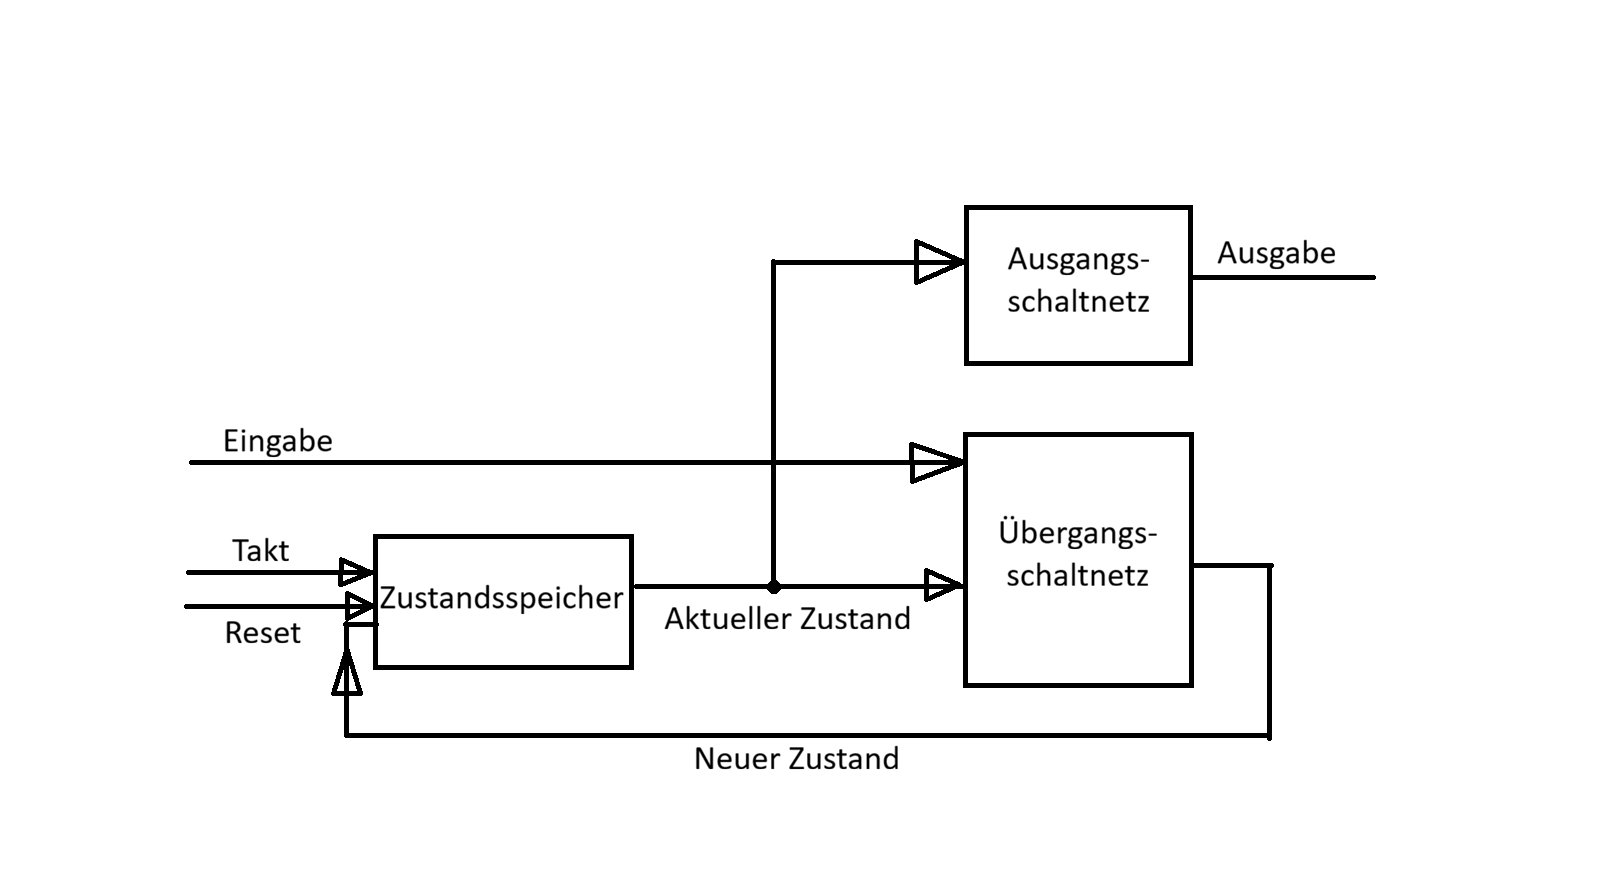
\includegraphics[scale=0.45]{Huffman.png}
	\end{center}
\end{figure}

\subsection{Zustandsspeicher der Schaltung implementieren}
Der Zustandsspeicher der Schaltung besteht aus 2 D-Flip-Flops, die die codierten Zustände des Modells speichern.
Die Belegung der Flip-Flops wird hier so gewählt, dass sie den Ausgangssignalen der Schaltung entspricht.
Das vereinfacht das Ausgangsschaltnetz.

\subsection{Übergangsschaltnetz implementieren}
Das Übergangsschaltnetz wird als boolsche Funktion aus der Wahrheitstabelle der Übergangsfunktion des Modells durch die KV-Minimierung ermittelt.
Die Tabelle und die verwendeten Diagramme sind auf der folge Seite abgebildet:
Die Wahrheitstabelle der Schaltung wird mittels der KV-Minimierung in boolsche Funktionen übersetzt.\\
Damit ergibt sich für k0 \rightarrow $(\overline{inOG}\cdot wunschOG)+(\overline{inOG}\cdot obergeschoss_o )$.\\
Und für k1 \rightarrow $(inOG\cdot wunschEG)+(inOG\cdot erdgeschoss_o )$

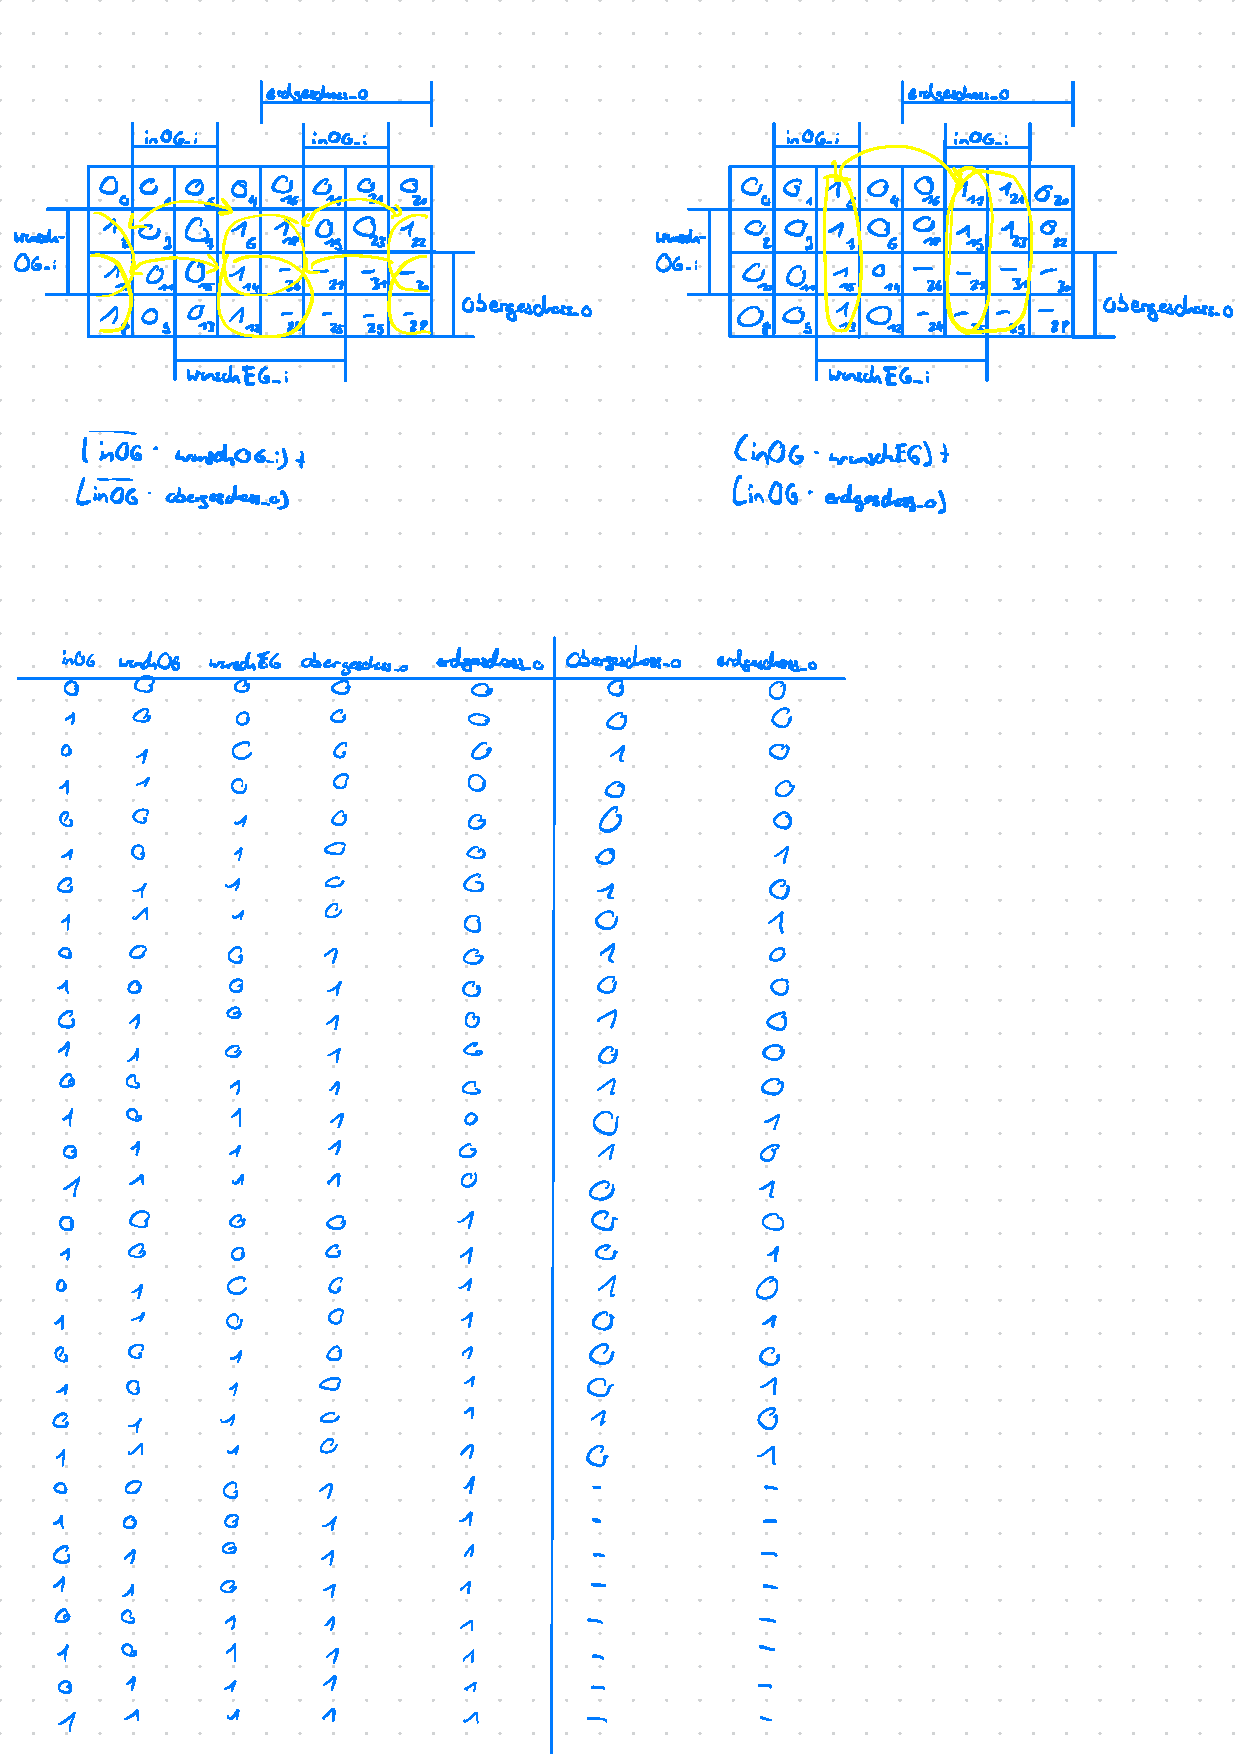
\includepdf[pages=-]{KV.pdf}




\subsection{Ausgangschaltnetz implementieren}

Da die Ausgangssignale identisch mit den Signalen der Zustandsspeicher sind, können diese direkt an die Ausgänge weitergeleitet werden

Der Ausgang k0 kann direkt zum Ausgang $erdgeschoss_o$ geleitet werden und der Ausgang k1 zum Ausgang $obergeschoss_o$

\subsection{Schaltplan zeichnen}
Die gesamte Schaltung bestehend aus Zustandsspeicher, Übergangsfunktion und Ausgangsschaltnetz
ist hier abgebildet:
Die Implementierung ist hier eingefügt:

	\begin{figure}[H]
		\begin{center}
			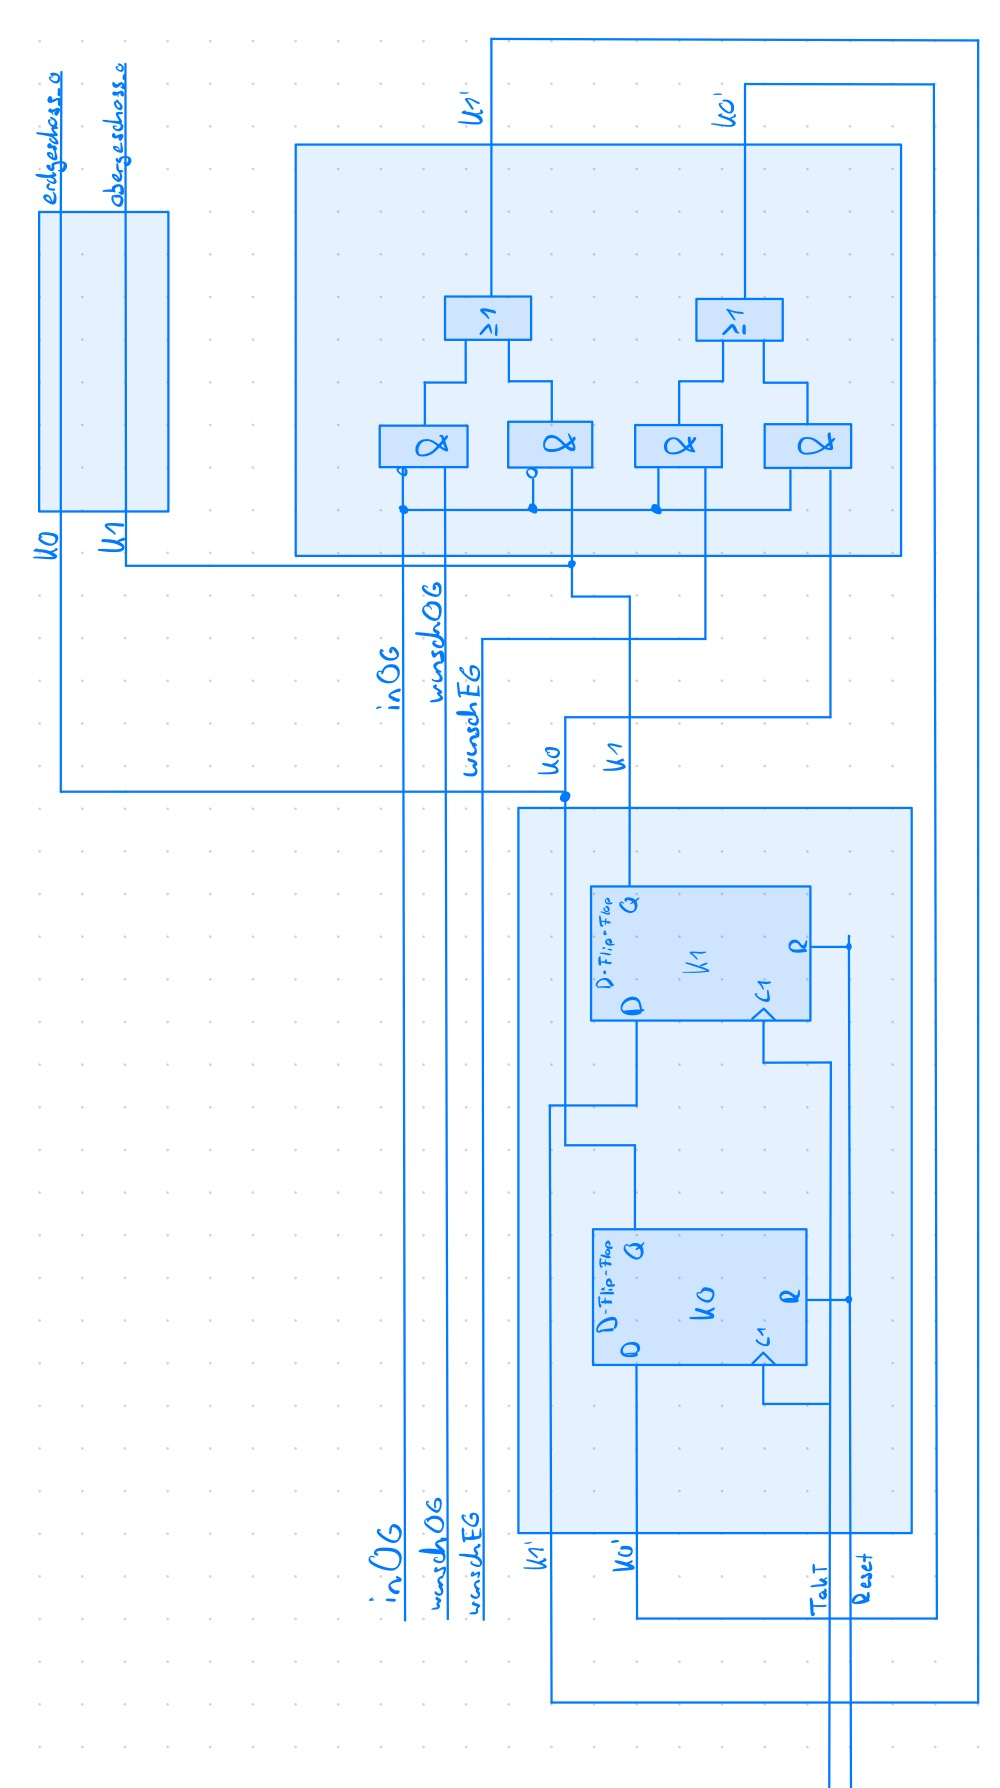
\includegraphics[scale=0.25,angle=270]{schaltung.jpeg}
		\end{center}
	\end{figure}


\section{Testdurchführung}
\subsection{Testfolgen ausführen}

Die Testfolgen sind nacheinander durchzuführen und jeder Schrift ist händisch abzuhaken

\begin{table}[H]
	\begin{tabular}{lllll|lll}
		clk & reset & $wunschEG_i$ & $wunschOG_i$ & \multicolumn{1}{l|}{inOG} & $erdgeschoss_o$ & $obergeschoss_o$ & OK\\ \hline
		0   & 1     & 0        & 0        & \multicolumn{1}{l|}{0}    & 0              & 0 &                \\
		0   & 0     & 0        & 0        & \multicolumn{1}{l|}{0}    & 0              & 0 &                \\
		1   & 0     & 0        & 0        & \multicolumn{1}{l|}{0}    & 0              & 0 &                \\
		0   & 0     & 0        & 0        & \multicolumn{1}{l|}{0}    & 0              & 0 &                \\
		0   & 0     & 0        & 1        & \multicolumn{1}{l|}{0}    & 0              & 0 &                \\ \hline
		1   & 0     & 0        & 1        & \multicolumn{1}{l|}{0}    & 0              & 1 &                \\
		0   & 0     & 0        & 1        & \multicolumn{1}{l|}{0}    & 0              & 1 &                \\
		0   & 1     & 0        & 1        & \multicolumn{1}{l|}{0}    & 0              & 0 & 
	\end{tabular}
\end{table}
Vor Beginn der Testfolge ist der Reset zu betätigen und seine in Testfolge 1 getestet Funktionalität zu verifizieren.
\begin{table}[H]
	\begin{tabular}{llllll}
		$wunschEG_i$ & $wunschOG_i$ & \multicolumn{1}{l|}{$inOG_i$} & $erdgeschoss_o$ & $obergeschoss_o$ & OK\\ \hline
		0          & 0          & \multicolumn{1}{l|}{0}      & 0             & 0 &               \\
		0          & 0          & \multicolumn{1}{l|}{1}      & 0             & 0 &               \\
		0          & 1          & \multicolumn{1}{l|}{1}      & 0             & 0 &               \\
		1          & 0          & \multicolumn{1}{l|}{0}      & 0             & 0 &               \\ \hline
		1          & 0          & \multicolumn{1}{l|}{1}      & 1             & 0 &               \\
		0          & 0          & \multicolumn{1}{l|}{1}      & 1             & 0 &               \\
		0          & 1          & \multicolumn{1}{l|}{1}      & 1             & 0 &               \\
		1          & 0          & \multicolumn{1}{l|}{1}      & 1             & 0 &               \\
		1          & 1          & \multicolumn{1}{l|}{1}      & 1             & 0 &               \\ \hline
		0          & 0          & \multicolumn{1}{l|}{0}      & 0             & 0 &               \\ \hline
		1          & 1          & \multicolumn{1}{l|}{1}      & 1             & 0 &               \\ \hline
		1          & 0          & \multicolumn{1}{l|}{0}      & 0             & 0 &               \\ \hline
		0          & 1          & \multicolumn{1}{l|}{0}      & 0             & 1 &               \\
		0          & 0          & \multicolumn{1}{l|}{0}      & 0             & 1 &               \\
		0          & 1          & \multicolumn{1}{l|}{0}      & 0             & 1 &               \\
		1          & 0          & \multicolumn{1}{l|}{0}      & 0             & 1 &               \\
		1          & 1          & \multicolumn{1}{l|}{0}      & 0             & 1 &               \\ \hline
		0          & 0          & \multicolumn{1}{l|}{1}      & 0             & 0 &               \\ \hline
		1          & 1          & \multicolumn{1}{l|}{0}      & 0             & 1 &               \\ \hline
		1          & 0          & \multicolumn{1}{l|}{1}      & 1             & 0 &               \\ \hline
		0          & 1          & \multicolumn{1}{l|}{0}      & 0             & 1 &               \\ \hline
		1          & 1          & \multicolumn{1}{l|}{1}      & 1             & 0 &               \\ \hline
		1          & 1          & \multicolumn{1}{l|}{0}      & 0             & 1 &               \\ \hline
		0          & 1          & \multicolumn{1}{l|}{1}      & 0             & 0 &               \\ \hline
	\end{tabular}
\end{table}

\newpage
\subsection{Gesamtergebnis}

\newpage

\section{Zweites System mit Fahrstuhlmodell}

Für das zweite System welches die implementierte Schaltung verwendet, wird ein Aufzugsmodell verwendet.
Dessen Schnittstellen entsprechen dem Steckbrettmodell und werden entsprechend der Aufgabenstellung verkabelt.
Da sich die Schaltungslogik im zweiten System nicht verändert steht beim Testen des zweiten Systems das Anschlusstesten im Vordergrund.
Dazu werden die in der Aufgabenstellung gegebenen Testziele und Testfolgen verwendet. Diese sind dem Anhang zu entnehmen.

\section{Anhang}

Fakultät 4 - Prof. Dr. Jan Bredereke - Entwurf digitaler Schaltungen - Laboraufgabe 1 - Fahrstuhlsteuerung


\includepdf[pages=-]{1 Fahrstuhlsteuerung auf dem Steckbrett.pdf}

\end{document}